\chapter{Supporting Information for Ab-initio Studies of Exciton Interactions of Cy5 Dyes}
\label{chap:ab-initio-SI}

%---------------------------------------------
\newpage % NOTE: The appendix title should be on its own page.
%---------------------------------------------

As Cy5 is a cationic dye, the presence of an explicit (chlorine) counter ion will likely affect the solvation and interaction energy. It was found that inclusion of the counter ion(s) resulted in a less negative solvation energy and a more negative interaction energy for the dimer structures and a more negative solvation energy for the Cy5 monomer (see \autoref{tab:cl-energies}). This does not necessarily suggest that the structure without the counter ion is more soluble, but instead because the vacuum structure is more stable with the counter ion, the solvent does not need to do as much to stabilize the charge.

\begin{table}[h]
\centering
\caption{Solvation energy and interaction energy of relaxed Cy5 H-dimers (flipped and stacked) and monomer for given basis sets and exchange-correlation (xc) functionals with explicit counter ion(s). The energies of the same structure optimized at the same level of theory without the counter ion(s) are also included for comparison.} \label{tab:cl-energies}
\begin{tabular}{|lll|p{15mm}|p{20mm}|}
\hline
\multicolumn{3}{|l|}{Structure}                                        & Solvation Energy (eV) & Interaction Energy (eV) \\ \hline
\multicolumn{1}{|l|}{Cy5 monomer}                & \multicolumn{1}{l|}{6-31+G(d,p)} & B3LYP   & -1.488        & --           \\ \hline
\multicolumn{1}{|l|}{Cy5 monomer + 1Cl$^{-}$}            & \multicolumn{1}{l|}{6-31+G(d,p)} & B3LYP   & -1.947        & --           \\ \hline
\multicolumn{1}{|l|}{H-dimer (flipped)}             & \multicolumn{1}{l|}{6-31+G(d,p)} & $\omega$B97-XD  & --          & -0.636         \\ \hline
\multicolumn{1}{|l|}{H-dimer (flipped) + 2Cl$^{-}$}         & \multicolumn{1}{l|}{6-31+G(d,p)} & $\omega$B97-XD  & --          & -0.665         \\ \hline
\multicolumn{1}{|l|}{\multirow{2}{*}{H-dimer (stacked)}}    & \multicolumn{1}{l|}{6-31+G(d,p)} & CAM-B3LYP & -4.638        & -0.069         \\ \cline{2-5} 
\multicolumn{1}{|l|}{}                     & \multicolumn{1}{l|}{6-31+G(d,p)} & $\omega$B97-XD  & -4.690        & -1.055         \\ \hline
\multicolumn{1}{|l|}{\multirow{2}{*}{H-dimer (stacked) + 2Cl$^{-}$}} & \multicolumn{1}{l|}{6-31+G(d,p)} & CAM-B3LYP & -3.322        & -0.088         \\ \cline{2-5} 
\multicolumn{1}{|l|}{}                     & \multicolumn{1}{l|}{6-31+G(d,p)} & $\omega$B97-XD  & -2.980        & -1.170         \\ \hline
\end{tabular}
\end{table}

The relaxed structure for oblique dimer with chlorine counter ions was also calculated using the 6-31+G(d,p) basis and $\omega$B97XD functional. Analysis of this structure with the KRM code (see \autoref{spectra-cl}) shows that it is not as good of fit as the oblique dimer without the chlorine counter ions. (The RMSE between the predicted spectrum of the oblique dimer without chlorine and experiment with this functional is 0.0514.)
\begin{figure}[h!]
  \centering
  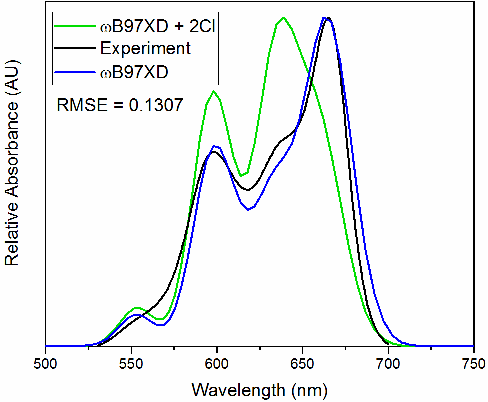
\includegraphics[width=0.8\linewidth]{figures/pub1/ob-dimer-Cl-wB97XD.pdf}
  \caption[Theoretical absorbance spectrum generated using KRM code for the oblique dimer with chlorine counter ions relaxed using $\omega$B97XD xc-functional compared to experimental absorbance of oblique dimer obtained by Cannon and oblique dimer without chlorine ions. RMSE value provided for quantification of difference.]{Theoretical absorbance spectrum generated using KRM code for the oblique dimer with chlorine counter ions relaxed using $\omega$B97XD xc-functional compared to experimental absorbance of oblique dimer obtained by \citet{Cannon2017} and oblique dimer without chlorine ions. RMSE value provided for quantification of difference.}\label{spectra-cl}
\end{figure}

As our method used a finite basis set, the overlap of basis functions can cause an increase in the effective basis set which in turn result in a lower energy solution to the Schrödinger equation. The difference in energy between the finite overlapping basis set and the theoretical infinite basis set is called basis set superposition error (BSSE). By comparing the energies and geometries of the systems optimized with a small basis set to those optimized using a large basis set, the amount of BSSE present can be qualitatively described. Using a series of basis sets and exchange-correlation functionals, the optimized geometries of the Cy5 monomer and H-dimer were compared to determine the extent of BSSE. 

\begin{table}[h]
\centering
\caption{Orientation of the relaxed Cy5 stacked H-dimer structures for given basis sets and exchange-correlation (xc) functionals including the zenith ($\theta$) and azimuth ($\phi$) angles for the vectors which lie along the long axis of the chromophores (arbitrarily labelled dye 1 and 2), the zenith ($\theta_{p}$) and azimuth ($\phi_{p}$) angles for the perpendicular vector which points in the direction of the methyl groups connected to the tertiary amine (see \autoref{3d-vectors} for a graphical representation of these vectors), and the centers of mass of the chromophores.} \label{tab:h-stacked-orientation}
\begin{tabular}{|p{20mm}|p{17mm}|l|l|c|c|c|ccc|}
\hline
\multirow{2}{*}{Basis Set} & xc- & \multirow{2}{*}{dye} & \multirow{2}{*}{$\theta$ (\textdegree)} & \multirow{2}{*}{$\phi$ (\textdegree)} & \multirow{2}{*}{$\theta_{p}$ (\textdegree)} & \multirow{2}{*}{$\phi_{p}$ (\textdegree)} & \multicolumn{3}{c|}{center of mass} \\ \cline{8-10} 
 & functional & & & & & & \multicolumn{1}{l|}{x (nm)} & \multicolumn{1}{l|}{y (nm)} & z (nm) \\ \hline
6-31+G & B3LYP & 1 & 71.00 & 173.64 & 93.93 & -97.64 & \multicolumn{1}{l|}{-0.033} & \multicolumn{1}{l|}{-0.006} & 0.411 \\ \cline{3-10} 
(d,p) & & 2 & 72.48 & 48.20 & 84.11 & 139.97 & \multicolumn{1}{l|}{0.033} & \multicolumn{1}{l|}{0.006} & -0.411 \\ \hline
6-31+G & CAM- & 1 & 72.77 & -179.77 & 95.74 & -91.47 & \multicolumn{1}{l|}{-0.013} & \multicolumn{1}{l|}{0.018} & 0.347 \\ \cline{3-10} 
(d,p) & B3LYP & 2 & 71.25 & 41.80 & 83.60 & 133.86 & \multicolumn{1}{l|}{0.013} & \multicolumn{1}{l|}{-0.018} & -0.347 \\ \hline
6-31+G & $\omega$B97- & 1 & 81.42 & -173.25 & 97.43 & -84.36 & \multicolumn{1}{l|}{0.008} & \multicolumn{1}{l|}{0.013} & 0.273 \\ \cline{3-10} 
(d,p) & XD & 2 & 78.15 & 35.08 & 81.03 & 126.92 & \multicolumn{1}{l|}{-0.008} & \multicolumn{1}{l|}{-0.013} & -0.273 \\ \hline
6-311++G & B3LYP & 1 & 69.90 & 179.28 & 92.62 & -91.62 & \multicolumn{1}{l|}{-0.053} & \multicolumn{1}{l|}{-0.023} & 0.488 \\ \cline{3-10} 
(2df,2pd) & & 2 & 75.83 & 43.05 & 92.71 & 132.39 & \multicolumn{1}{l|}{0.053} & \multicolumn{1}{l|}{0.023} & -0.488 \\ \hline
6-311++G & CAM- & 1 & 72.75 & -179.44 & 95.47 & -91.06 & \multicolumn{1}{l|}{-0.012} & \multicolumn{1}{l|}{0.016} & 0.348 \\ \cline{3-10} 
(2df,2pd) & B3LYP & 2 & 71.23 & 41.41 & 83.44 & 133.52 & \multicolumn{1}{l|}{0.012} & \multicolumn{1}{l|}{-0.016} & -0.348 \\ \hline
6-311++G & $\omega$B97- & 1 & 80.80 & -173.96 & 97.28 & -85.13 & \multicolumn{1}{l|}{0.008} & \multicolumn{1}{l|}{0.004} & 0.267 \\ \cline{3-10} 
(2df,2pd) & XD & 2 & 78.14 & 35.71 & 83.95 & 126.95 & \multicolumn{1}{l|}{-0.008} & \multicolumn{1}{l|}{-0.004} & -0.267 \\ \hline
\end{tabular}
\end{table}

\begin{table}[h]
\centering
\caption{Orientation of the relaxed Cy5 flipped H-dimer structures for given basis sets and exchange-correlation (xc) functionals including the zenith ($\theta$) and azimuth ($\phi$) angles for the vectors which lie along the long axis of the chromophores (arbitrarily labelled dye 1 and 2), the zenith ($\theta_{p}$) and azimuth ($\phi_{p}$) angles for the perpendicular vector which points in the direction of the methyl groups connected to the tertiary amine (see \autoref{3d-vectors} for a graphical representation of these vectors), and the centers of mass of the chromophores.} \label{tab:h-flipped-orientation}
\begin{tabular}{|p{20mm}|p{17mm}|l|l|c|c|c|ccc|}
\hline
\multirow{2}{*}{Basis Set} & xc- & \multirow{2}{*}{dye} & \multirow{2}{*}{$\theta$ (\textdegree)} & \multirow{2}{*}{$\phi$ (\textdegree)} & \multirow{2}{*}{$\theta_{p}$ (\textdegree)} & \multirow{2}{*}{$\phi_{p}$ (\textdegree)} & \multicolumn{3}{c|}{center of mass} \\ \cline{8-10} 
 & functional & & & & & & \multicolumn{1}{c|}{x (nm)} & \multicolumn{1}{c|}{y (nm)} & z (nm) \\ \hline
6-31+G & B3LYP & 1 & 89.72 & 11.53 & 79.78 & 101.58 & \multicolumn{1}{l|}{-0.176} & \multicolumn{1}{l|}{-0.027} & 0.315 \\ \cline{3-10} 
(d,p) & & 2 & 94.92 & 29.68 & 106.35 & 121.06 & \multicolumn{1}{l|}{0.176} & \multicolumn{1}{l|}{0.027} & -0.315 \\ \hline
6-31+G & CAM- & 1 & 94.30 & 20.99 & 85.06 & 110.62 & \multicolumn{1}{l|}{-0.155} & \multicolumn{1}{l|}{-0.033} & 0.246 \\ \cline{3-10} 
(d,p) & B3LYP & 2 & 93.96 & 19.61 & 104.34 & 110.59 & \multicolumn{1}{l|}{0.155} & \multicolumn{1}{l|}{0.033} & -0.246 \\ \hline
6-31+G & $\omega$B97- & 1 & 95.08 & 20.31 & 85.37 & 109.90 & \multicolumn{1}{l|}{-0.139} & \multicolumn{1}{l|}{-0.037} & 0.208 \\ \cline{3-10} 
(d,p) & XD & 2 & 94.77 & 20.05 & 101.54 & 111.01 & \multicolumn{1}{l|}{0.139} & \multicolumn{1}{l|}{0.037} & -0.208 \\ \hline
6-311++G & B3LYP & 1 & 89.84 & 9.56 & 79.50 & 99.59 & \multicolumn{1}{l|}{-0.228} & \multicolumn{1}{l|}{-0.040} & 0.383 \\ \cline{3-10} 
(2df,2pd) & & 2 & 97.12 & 31.23 & 106.69 & 123.27 & \multicolumn{1}{l|}{0.228} & \multicolumn{1}{l|}{0.040} & -0.383 \\ \hline
6-311++G & CAM- & 1 & 94.25 & 20.87 & 84.98 & 110.49 & \multicolumn{1}{l|}{-0.155} & \multicolumn{1}{l|}{-0.033} & 0.245 \\ \cline{3-10} 
(2df,2pd) & B3LYP & 2 & 93.93 & 19.79 & 104.16 & 110.75 & \multicolumn{1}{l|}{0.155} & \multicolumn{1}{l|}{0.033} & -0.245 \\ \hline
6-311++G & $\omega$B97- & 1 & 95.13 & 20.22 & 85.47 & 109.81 & \multicolumn{1}{l|}{-0.138} & \multicolumn{1}{l|}{-0.036} & 0.208 \\ \cline{3-10} 
(2df,2pd) & XD & 2 & 94.68 & 20.17 & 101.86 & 111.13 & \multicolumn{1}{l|}{0.138} & \multicolumn{1}{l|}{0.036} & -0.208 \\ \hline
\end{tabular}
\end{table}

Except for the case of the B3LYP exchange-correlation functional (\autoref{spectra-bsse} a and b), there is good agreement of the spectra generated using the H-dimer structures relaxed using the 6-311++G(2df,2pd) and 6-31+G(d,p) basis sets, suggesting the degree of BSSE present in the 6-31+G(d,p) basis set does not impact the energy or structure enough to justify using the 6-311++G(2df,2pd) basis set. The disagreement occurs in the B3LYP case due to the absence of long range and/or dispersion correction in the exchange-correlation functional, showing failure to accurately estimate the inter-dye interactions. These results suggest that the magnitude of basis set BSSE in the small basis set does not significantly impact the resulting energies enough to justify using the large basis set, so the small basis set was used for further calculations to reduce computational time. 
\begin{figure}[h!]
  \centering
  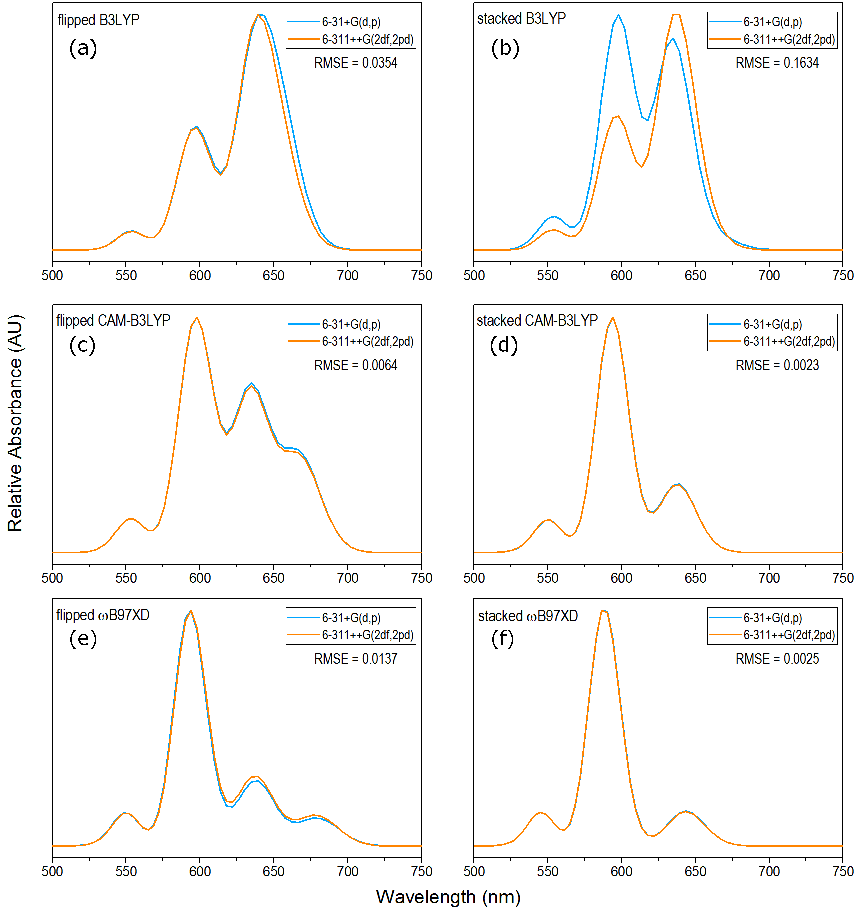
\includegraphics[width=0.8\linewidth]{figures/pub1/H-dimersall-af.pdf}
  \caption{Comparison of basis set effect on theoretical absorbance spectra of (a)(c)(e) the flipped and (b)(d)(f) stacked H-dimer structures predicted using KRM code. With the exception of the stacked structure relaxed using (b) B3LYP, the spectra show significant overlap for the 6-311++G(2df,2pd) and 6-31+G(d,p) basis sets suggesting the smaller basis set is adequate. RMSE value provided for quantification of difference.}\label{spectra-bsse}
\end{figure}

\begin{figure}[h!]
  \centering
  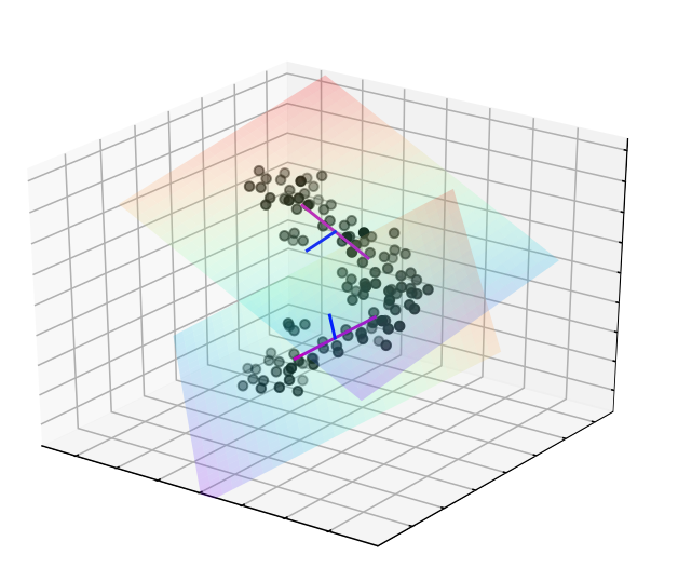
\includegraphics[width=0.8\linewidth]{figures/pub1/fitting-vectors.pdf}
  \caption{Graphic showing the vector fit to long axes of the molecules (magenta), the plane of the molecule (rainbow), and the perpendicular vector pointing in the direction of the tertiary amine (blue). }\label{3d-vectors}
\end{figure}
In order to succinctly represent the relative orientation of the dyes in a dimer structure, the dye molecules are simplified to vectors. To calculate these vectors, the atom positions in dye molecules are fit to a plane, using the method of least squares, and a vector, using a singular value decomposition (\autoref{3d-vectors}). As the molecules are longer than their width, only the vector which lies along the long axis of the molecule is used to represent the molecule in the KRM code. A vector which points in the direction of the methyl groups connected to the tertiary amine, lies in the plane of the molecule, and is perpendicular to the long axis of the molecule was also defined to provide the absolute orientation of the chromophores. The zenith and azimuth angles ($\theta$ and $\phi$, respectively) for these vectors for the H- and oblique dimers in spherical coordinates are given in \autoref{tab:h-stacked-orientation}, \autoref{tab:h-stacked-orientation}, and \autoref{tab:ob-orientation}.
\begin{figure}[h!]
  \centering
  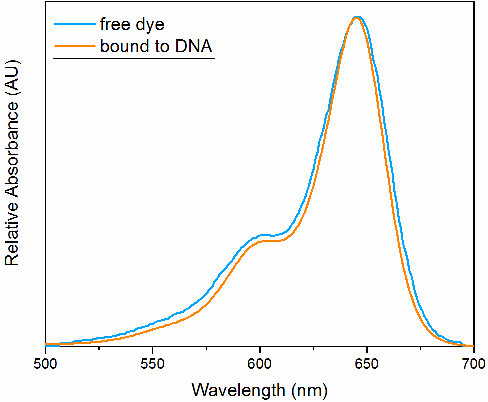
\includegraphics[width=0.8\linewidth]{figures/pub1/free-vs-bound-cy5.pdf}
  \caption[Comparison of absorbance spectra of Cy5 dye when free in solution and when bound to duplex DNA.]{Comparison of absorbance spectra of Cy5 dye when free in solution and when bound to duplex DNA \cite{Cannon2017, thermofisher}.}\label{spectra-free-bound}
\end{figure}

Assuming that the DNA scaffold does not have a large impact on the electrostatic environment of the Cy5 dyes may be a gross oversimplification; however, this assumption is supported by the observation that the absorbance spectrum of Cy5 does not exhibit a shift in absorbance maxima or noticeable change in vibronic structure when bound to DNA (see \autoref{spectra-free-bound}).


\begin{table}[h]
\centering
\caption{Orientation of the Cy5 oblique dimer optimized using the 6-31+G(d,p) and specified exchange-correlation (xc) functionals including the zenith ($\theta$) and azimuth ($\phi$) angles for the vectors which lie along the long axis of the chromophores (arbitrarily labelled dye 1 and 2), the zenith ($\theta_{p}$) and azimuth ($\phi_{p}$) angles for the perpendicular vector which points in the direction of the methyl groups connected to the tertiary amine (see \autoref{3d-vectors} for a graphical representation of these vectors), and the centers of mass of the chromophores.} \label{tab:ob-orientation}
\begin{tabular}{|l|l|l|l|l|l|lll|}
\hline
\multirow{2}{*}{xc-functional} & \multirow{2}{*}{dye} & \multirow{2}{*}{$\theta$ (\textdegree)} & \multirow{2}{*}{$\phi$ (\textdegree)} & \multirow{2}{*}{$\theta_{p}$ (\textdegree)} & \multirow{2}{*}{$\phi_{p}$ (\textdegree)} & \multicolumn{3}{c|}{center of mass} \\ \cline{7-9} 
 & & & & & & \multicolumn{1}{l|}{x (nm)} & \multicolumn{1}{l|}{y (nm)} & z (nm) \\ \hline
\multirow{2}{*}{B3LYP} & 1 & 105.67 & -21.32 & 118.72 & 45.21 & \multicolumn{1}{l|}{0.507} & \multicolumn{1}{l|}{-0.343} & 0.308 \\ \cline{2-9} 
 & 2 & 29.20 & 33.96 & 147.32 & -137.60 & \multicolumn{1}{l|}{-0.507} & \multicolumn{1}{l|}{0.343} & -0.308 \\ \hline
\multirow{2}{*}{CAM-B3LYP} & 1 & 103.82 & -18.46 & 111.98 & 30.32 & \multicolumn{1}{l|}{0.495} & \multicolumn{1}{l|}{-0.282} & 0.313 \\ \cline{2-9} 
 & 2 & 21.97 & 32.08 & 159.01 & -148.70 & \multicolumn{1}{l|}{-0.495} & \multicolumn{1}{l|}{0.282} & -0.313 \\ \hline
\multirow{2}{*}{$\omega$B97-XD} & 1 & 100.96 & -13.05 & 11.72 & 5.39 & \multicolumn{1}{l|}{0.506} & \multicolumn{1}{l|}{-0.235} & 0.325 \\ \cline{2-9} 
 & 2 & 19.55 & 33.20 & 109.59 & -151.56 & \multicolumn{1}{l|}{-0.506} & \multicolumn{1}{l|}{0.235} & -0.325 \\ \hline
\end{tabular}
\end{table}

The structure of the oblique dimer was also relaxed using the long range dispersion correction implemented by \citet{Grimme2006}. Two- (D2) and three-body (D3) dispersion effects have been considered, the latter also includes rational damping according to the formula of Becke and Johnson (BJ-damping) \cite{Grimme2011}. It was found that the absorbance spectra predicted using the KRM model are not more similar to experiment than $\omega$B97XD (see \autoref{spectra-d2d3}). Interestingly, however, the oblique dimer structures optimized using dispersion-corrected B3LYP (D2 and D3-BJ) are more plane-parallel than those optimized using any other method, which may mean that this method models pi-stacking, which should require parallel stacking of the conjugated bonds, better than other dispersion-corrected methods.

\begin{figure}[h!]
  \centering
  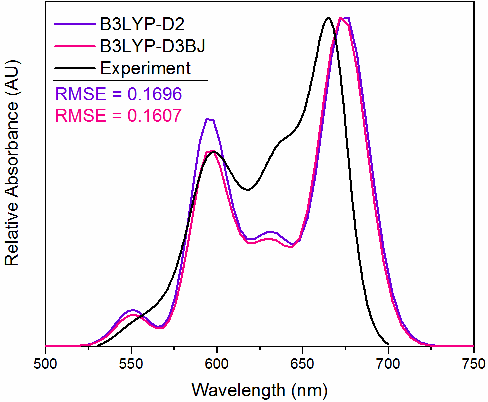
\includegraphics[width=0.8\linewidth]{figures/pub1/ob-dimer-B3LYP-D3andD2.pdf}
  \caption[Comparison of theoretical absorbance spectrum generated using KRM code for the oblique dimer structures relaxed using B3LYP-D2 and B3LYP-D3BJ xc-functionals compared to experimental absorbance of oblique dimer obtained by Cannon. RMSE values provided for quantification of difference.]{Comparison of theoretical absorbance spectrum generated using KRM code for the oblique dimer structures relaxed using B3LYP-D2 and B3LYP-D3BJ xc-functionals compared to experimental absorbance of oblique dimer obtained by \citet{Cannon2017}. RMSE values provided for quantification of difference.}\label{spectra-d2d3}
\end{figure}

\begin{table}[h]
\centering
\caption{Structural information for Cy5 monomers optimized with given basis set and exchange correlation (xc) functionals, showing little significant difference between structures. The molecule length is measured as the greatest distance between any two atoms in the molecule and the methine chain is the greatest distance between carbon atoms in the methine chain. } \label{tab:structure}
\begin{tabular}{|p{25mm}|p{25mm}|p{22mm}|p{28mm}|p{30mm}|}
\hline
Basis Set & xc-functional & Molecule \newline length (\AA) & Methine chain \newline length (\AA) & Average C=C \newline bond length (\AA) \\ \hline
6-31+G(d,p) & B3LYP & 18.698 & 7.436 & 1.398 \\ \hline
6-31+G(d,p) & CAM-B3LYP & 18.572 & 7.386 & 1.392 \\ \hline
6-31+G(d,p) & $\omega$B97-XD & 18.495 & 7.365 & 1.393 \\ \hline
6-311++G \newline (2df,2pd) & B3LYP & 18.616 & 7.403 & 1.391 \\ \hline
6-311++G \newline (2df,2pd) & CAM-B3LYP & 18.480 & 7.349 & 1.386 \\ \hline
6-311++G \newline (2df,2pd) & $\omega$B97-XD & 18.396 & 7.328 & 1.387 \\ \hline
\end{tabular}
\end{table}

\begin{figure}[h!]
  \centering
  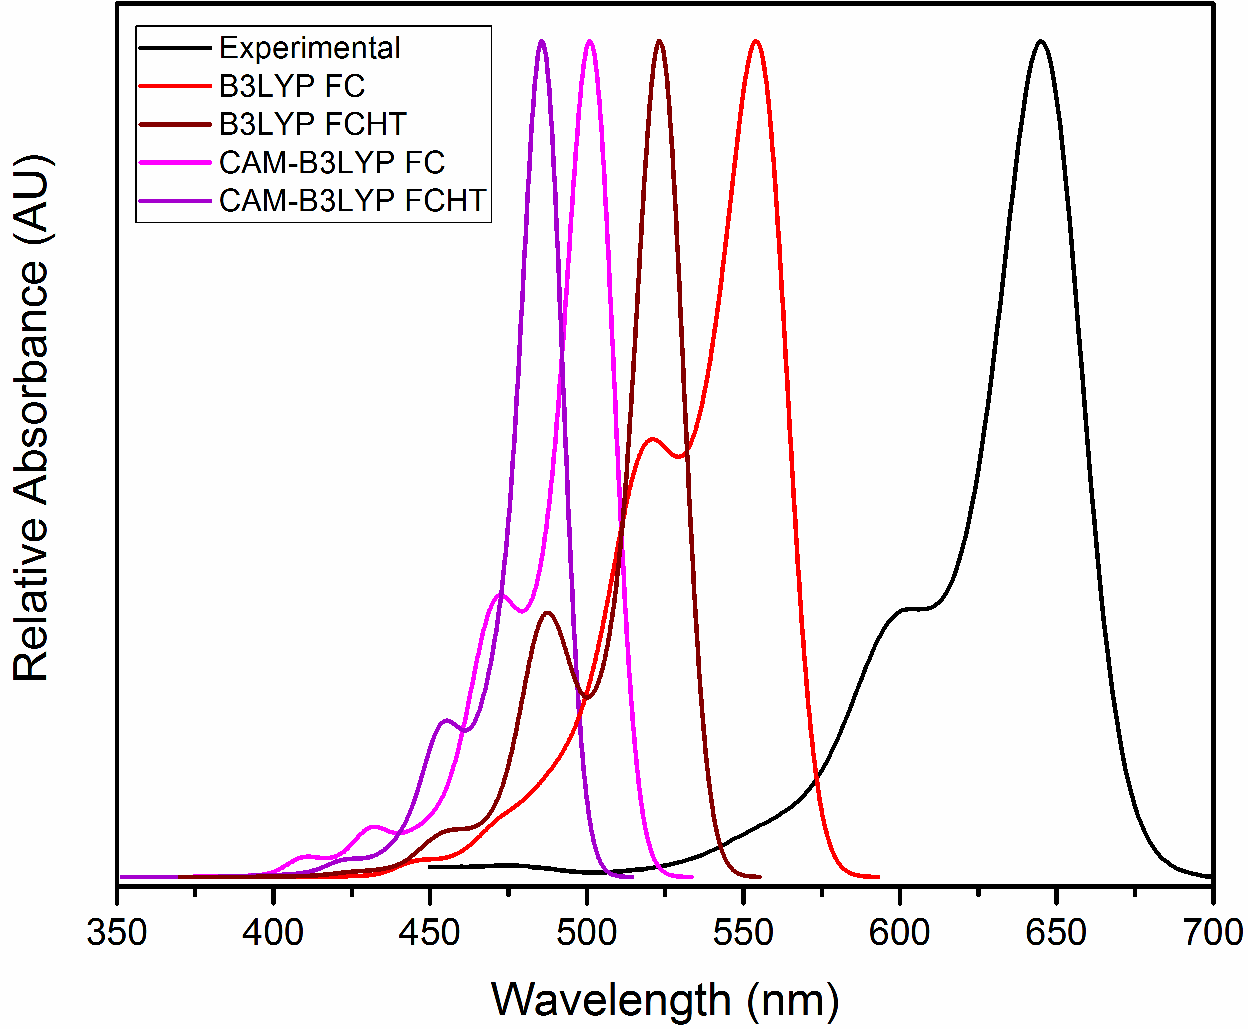
\includegraphics[width=0.8\linewidth]{figures/pub1/FCHT-vac.pdf}
  \caption[Comparison of Cy5 monomer spectra generated using the FC approximation with and without the HT approximation to experimental spectrum obtained by Cannon. Comparison of the vacuum spectra to those obtained using a solvent model (\autoref{spectra-fc-pcm} and \autoref{spectra-fcht-pcm}) show that the bathochromic shift induced by the solvent provides a more accurate prediction of the maximum absorbance]{Comparison of Cy5 monomer spectra generated using the FC approximation with and without the HT approximation to experimental spectrum obtained by \citet{Cannon2017}. Comparison of the vacuum spectra to those obtained using a solvent model (\autoref{spectra-fc-pcm} and \autoref{spectra-fcht-pcm}) show that the bathochromic shift induced by the solvent provides a more accurate prediction of the maximum absorbance}\label{spectra-vac}
\end{figure}